\documentclass[12pt]{amsart}
\usepackage[utf8]{inputenc}
\usepackage[a4paper,margin=1in,footskip=0.25in]{geometry}

% See geometry.pdf to learn the layout options. There are lots.
\geometry{letterpaper}                   % ... or a4paper or a5paper or ... 
%\geometry{landscape}                % Activate for for rotated page geometry
%\usepackage[parfill]{parskip}    % Activate to begin paragraphs with an empty line rather than an indent
\usepackage{float}
\usepackage{graphicx}
\usepackage{amssymb}
\usepackage{epstopdf}
\usepackage{amsmath}
\newtheorem{thm}{Theorem}
%\usepackage{algorithm}
\usepackage{subfig}
\usepackage[authoryear]{natbib}
%\usepackage{subcaption}
\usepackage[ruled,vlined,linesnumbered]{algorithm2e}
\linespread{1}
\usepackage{comment}
\usepackage{booktabs}
\usepackage[colorlinks=true,linkcolor=blue, citecolor=blue]{hyperref}%

\usepackage{listings}
\usepackage{color}

\definecolor{dkgreen}{rgb}{0,0.6,0}
\definecolor{gray}{rgb}{0.5,0.5,0.5}
\definecolor{mauve}{rgb}{0.58,0,0.82}

\lstset{frame=tb,
  language=python,
  aboveskip=3mm,
  belowskip=3mm,
  showstringspaces=false,
  columns=flexible,
  basicstyle={\small\ttfamily},
  numbers=none,
  numberstyle=\tiny\color{gray},
  keywordstyle=\color{blue},
  commentstyle=\color{dkgreen},
  stringstyle=\color{mauve},
  breaklines=true,
  breakatwhitespace=true,
  tabsize=3
}

\def\THM#1{\textcolor[RGB]{23,117,67}{[#1]}}
\def\Peter#1{\textcolor[RGB]{224, 123, 57}{[#1]}}

\begin{document}
\author{Chris Chen}
\author{Bolun Liu}
\author{Yueqi Xu}
\title{STAT 423 Final Project}

\maketitle
\section{Introduction}
\label{sec: intro}
Perfumes can be defined as substances that emit and diffuse a pleasant and fragrant odor (\cite{perfume}). The manufacture and use of perfumes goes back thousands of years. Ancient Egyptians, Indians, and Chinese used plants, gums, and resins for fragrance in religious rites (\cite{perfume}). Until the nineteenth century, perfumes were usually made from natural aromatic chemicals and essential oils. In the modern age, with the development of chemical technology, most perfumes become synthetic, and the number of commercial perfumes surged significantly. With an overwhelming amount of perfumes in the markets, it is often hard for consumers to identify the perfume that best fits their demands. Moreover, given the perfumes' high retail prices, a false purchase can lead to great loss of money. In this project, we are interested in answering the following questions in order to quantify the relationships between perfume brand, customer ratings, $...$, etc. and retail prices and to assist consumers to better their purchases. The concerning questions are:

\begin{enumerate}
    \item Does the prestige of the brands contribute the most of the perfume's retail price? Namely, does bigger
brands typically cost more?
\item Does the customer rating contribute the most of the perfume's retail price? Namely, does a good perfume typically cost more?
\item From the perfume enthusiasts' perspective, does the perfume's department or scent generally lead to difference in retail prices? 
\end{enumerate}

\section{Methodology}

\subsection{Perfume Data set}
To investigate the above questions, we will analyze a data set of perfumes for female, male, and unisex, which is collected from a lifestyle shopping destination in Saudi Arabia called noon. The data set contains a collection of 1,002 perfumes, specified with
product parameters including retail price, brand, volume, fragrance concentration, department, scent, base notes, and middle notes, as well as retail information including retail company, customer \& retailer rating, and grand selling amount. The original data set can be found in \url{https://www.kaggle.com/monirahabdulaziz/noon-perfume?select=noon_perfumes_dataset.csv}. 

\subsubsection{Data Cleaning} The first step is to generally clean the original data and to prepare it for further analysis. The original data does not contain any missing values and \texttt{NA}s, which is great, yet it contains quite a lot of typos which need to be addressed. The original data seems to be directly crawled from the \textit{noon} web page. As a result, some of the same covariates are categorized by different names and languages (English, Arabian, Latin, etc.). Moreover, the web page crawling also induced multiple data points with nonsense perfume brands and notes. For instance, for several perfume data points, the famous cosmetic brand Yves Saint Laurent (often abbreviated into YSL) was considered as three different brands separately, which does not make sense. After solving the language and crawling-induced issues, the data set is reduced to 889 data points.

\subsubsection{Merging Categorical Covariates}

\begin{table}[!ht]
    \centering
    \renewcommand{\arraystretch}{1.2}
        \begin{tabular}{ c c c }
        \hline
             \textbf{Variable} & \textbf{Data Type} & \textbf{Description} \\ \hline
             \texttt{old\_price} & Quantitative & Perfume prices in USD \\  
             \texttt{ml} &Quantitative & Volume of perfumes in ml \\
             \texttt{item\_rating} & Quantitative & Customers’ ratings of perfume \\
             \texttt{seller\_rating} & Quantitative & Customers' ratings of seller \\
             \texttt{is\_EDT} & Categorical & The perfume’s concentration: EDP or EDT \\
             \texttt{num\_sel\_ratings} & Quantitative & Number of customers’ ratings on the seller \\
             \texttt{big\_brand} & Categorical & Whether perfume belongs to \emph{big brand}: 0 (no) or 1 (yes) \\
             \texttt{is\_noon} & Categorical & Whether perfume sold by \emph{noon}: 0 (no) or 1 (yes) \\
             \texttt{comp} & Quantitative & Complexity of perfume nodes \\
             \texttt{scent} & Categorical & Perfume scent \\
             \texttt{unisex} & Categorical & Perfume department (women/men/unisex)\\
             \hline
        \end{tabular}
 \vspace{10pt}
 \caption{Summary of the covariates we will consider in later regression analysis.}
\label{tab:1}
\end{table}

The second step is to reasonably merge the multiple levels of the categorical variables to improve the interpretation of our future regression models. We consider merging and truncating the following covariates:

\begin{enumerate}
    \item \texttt{brand} is a nominal categorical covariate, which originally contain 148 levels. Given the large amount of brands in the data set, we will impute the perfume brand into a binary categorical covariate \texttt{big\_brand} in the following manner. For a perfume brand with more than 10 individual perfumes in the data set, we will consider it as famous and popular, and take its binary covariate \texttt{big\_brand} as 1. Correspondingly, for a perfume brands with less than 10 individual perfumes, we will consider it as a niche brand, and take the indicator as 0.
    \item \texttt{seller} is a nominal categorical covariate, which originally contains 115 levels. We observed that over two thirds of \texttt{Seller} are directly affiliated with the \textit{noon} website (think it as \textit{Amazon's Choice}) and the rest come from a large variety of individual sellers. Thus, we will convert \texttt{Seller} into a binary covariate called \texttt{is\_noon}. If the perfume is sold by the \texttt{noon} official, we will take the indicator as 1, and 0 otherwise.
    \item \texttt{ml} is a discrete quantitative covariate indicating the perfume's volume. We will exclude the perfumes with volume $\leq 5$ml to remove the perfume samples/testers, as they are often free as giveaway subjected to purchase.
    \item \texttt{base\_note} and \texttt{middle\_note} are two nominal categorical covariates. First, we noticed that there exists several hierarchical structures in the covariate levels, for instance,  \texttt{Bulgarian Rose} and \texttt{Rose}, \texttt{Africa Orange Flower} and \texttt{Orange Blossom}, etc. We will manually merge all lower branches of the same hierarchy to the highest one. Moreover, since the levels of base and middle note are numerous, we will summarize the two categorical variables with one discrete quantitative covariate called \texttt{comp}, which represents the complexity of the perfume note. Namely, for a perfume $i$ we define
    \[\texttt{comp}_i \equiv \text{Total \# of unique note in }  \texttt{base\_note}_i \text{ and } \texttt{middle\_note}_i \;.\]
    We will explain in later sections our motivations of imputing covariate \texttt{comp}.
\end{enumerate}

After the above imputations, we obtained the variables in Table \ref{tab:1} as potential covariates of our regression model.

\subsection{Statistical Analysis}

We use the outcome variable \texttt{old\_price} and the ten covariates to perform a linear regression analysis. All analysis are conducted with the statistical computing software \texttt{R 4.1.2} (\cite{R}) and the IDE \texttt{Rstudio} (\cite{rstudio}) on macOS Big Sur Version 11.6. The default significant level is $\alpha = 0.05$ if not suggested otherwise.

\subsubsection{Exploratory Data Analysis}

We are first interested in investigating if there are any outliers in the data set. To do this, we fitted our data set with the full model and plot the fitted Cook's distance in Figure \ref{fig1}. 
\begin{figure}[H]
    \centering
    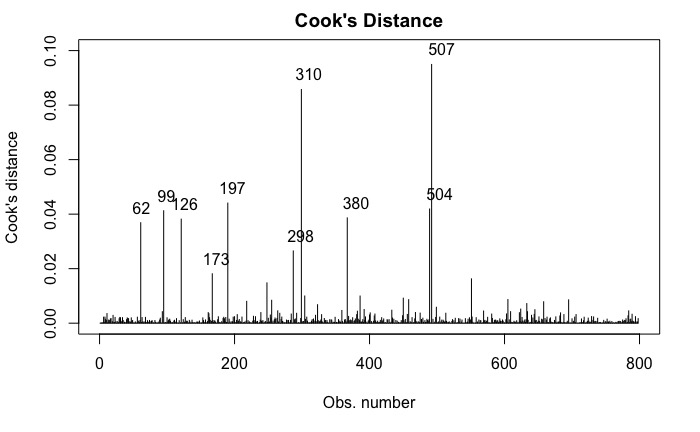
\includegraphics[width = 0.8\linewidth]{423f1.jpg}
    \caption{The fitted Cook's distance of the full model.}
    \label{fig1}
\end{figure}
From the plot we can observe that there are several data points with Cook's distances that are systematically higher. By the rule of thumb, since the highest distance is still smaller than 0.25, in general the outlier effect should not be considered as significant. Yet we are still interested in understanding what the outliers represent for and if they are induced by several covariates of interests. We found out that, the significant outliers in Figure \ref{fig1} are highly correlated with the retail prices. For instance, data points with the top three retail prices, namely data point 507, 504, and 197, all have some of the highest Cook's distances. With the average retail price of the perfumes around \$300, a perfume that is sold for over \$2000 is probably a special edition and will not fit well with the standard economic model we will later use to explain the regression result. Thus we consider the perfumes with high retail prices statistically invalid in our analysis and we shall truncate the data set by removing all data points with $\texttt{old\_price} \geq 930$. 

Our next step is to explore if there are potential interactions between the covariates. We will first investigate all possible two way interactions. To do this, we first plot the all the two way correlations between the covariates in Figure \ref{fig2} below. 
\begin{figure}[H]
    \centering
    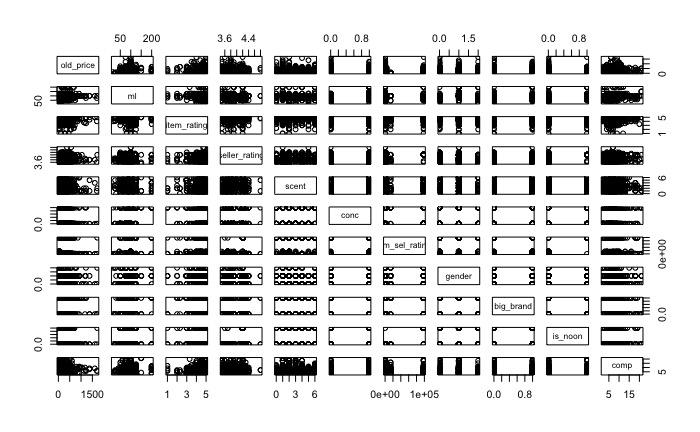
\includegraphics[width = \linewidth]{423f2.jpg}
    \caption{All possible two way interactions between outcome variable and the ten covariates.}
    \label{fig2}
\end{figure}
As we can observe from the plot, for correlations involved with quantitative covariates/outcome variable, there haven't been a significant linear trend or correlation. For categorical covariates, the data points seem to uniformly distributed across all levels of the covariates. We can then conclude roughly from the plot that there might not be significant two way interactions in the linear model of interest. Indeed, by computation in \texttt{R}, we found out that a two-way interaction is significant only if it is interacted with the covariate \texttt{big\_brand}. We argue that the significant interactions all result from the great importance of the covariate \texttt{big\_brand} in the regression model, and thus it is not appropriate to keep such two-way interactions in our analysis.

What about multiple-way interactions? Since the original data set contains a variety of categorical variables with multiple levels, especially with \texttt{base\_note} and \texttt{middle\_note}, we argue that enumerating and testing all possible multiple-way interactions can be intractable and will lead to difficulties in further model analysis and interpretation. Recall that, based on the two note covariates, we have impute a new covariate \texttt{comp} to quantify the complexity of perfume. We argue that it can be considered as a pseudo covariate to account for the multiple-way interactions between the perfume note levels. The idea is that, if there do exist multiple significant multiple-way interactions between the notes, and they all contribute to the retail prices in the same direction (positive or negative), the covariate \texttt{comp} should be significant, in such a way the complexity of the perfume will account for the interactions between the variety of the notes. We argue that the covariate \texttt{comp} will provide us with a convenient handle to incorporate multiple-way interactions, to simplify our model, and to enhance our model interpretability. 

\subsubsection{Model Selection}

By the analysis above, we decided not to consider any two-way interactions and to concentrate all possible multiple-way interaction in the complexity covariate. Our model is hence reduced to an additive model with ten covariates. We then perform a linear regression with step-wise backward strategy to find the optimal model with respected to criterion such as RSE, $R^2$, MSE, Generalized Error, Marlow's $C_p$, AIC, and BIC. For each step of model reduction, we attempted to remove the most insignificant covariates. Below are some of the models we evaluated in our model selection:
\begin{lstlisting}
# Full model with outliers
lm.1 = lm(price ~ ., data = perfume_original)
# Full model with outliers removed
lm.2 = lm(price ~ ., data = perfume)
# Further removing seller
lm.3 = lm(price ~ . - is_noon, data = perfume) 
# Further removing item_rating
lm.4 = lm(price ~ . - is_noon - item_rating, data = perfume)
# Further removing num_sel_ratings
lm.5 = lm(price ~ . - is_noon - item_rating - num_sel_ratings, data = perfume)
\end{lstlisting}
Their corresponding model evaluation criterion are listed in Table \ref{tab2} below. We can first confirm that, by removing the outliers, we do arrive at a better model fitting, with substantially better results in all criterion we considered. Then, after the model selection procedure, we consider \texttt{lm.5} as the most appealing model, which has a comparable $R^2$ value and the best AIC and BIC values. 

\begin{table}[H]
    \centering
    \renewcommand{\arraystretch}{1.2}
        \begin{tabular}{ c c c c c c c c}
            \hline
             \textbf{Model} & \textbf{RSE} & $\boldsymbol{R}^2$ & \textbf{MSE} & \textbf{GE} & $\boldsymbol{C}_p$ & \textbf{AIC} & \textbf{BIC}  \\ \hline
             lm.1 & $216.3359$ & $0.1194184$ & $45804.19$ & $1994.036$ & $47798.23$ & $10864.87$ & $10949.14$ \\
             lm.2 & $175.1131$ & $0.1754292$ & $\textbf{29999.69}$ & $1329.843$ & $31993.73$ & $10343.11$ & $10427.07$ \\
             lm.3 & $175.1453$ & $0.1751258$ & $30049.85$ & $1252.077$ & $31926.59$ & $10342.42$ & $10421.71$ \\
             lm.4 & $\textbf{175.0719}$ & $\textbf{0.1758177}$ & $30063.75$ & $1172.838$ & $31823.19$ & $10340.78$ & $10415.41$ \\
             lm.5 & $175.1381$ & $0.1751940$ & $30125.62$ & $\textbf{1095.477}$ & $\textbf{31767.77}$ & $\textbf{10340.39}$ & $\textbf{10410.36}$ \\ \hline
        \end{tabular}
 \vspace{10pt}
 \caption{Summary of the model goodness-of-fit criterion for the five models above. The bold number represents the optimal criterion values.}
\label{tab2}
\end{table}

\subsubsection{Improving Model Interpretability} There are still a considerable amount of covariates and levels in the optimal model and we are interested in further reducing the covariates and improving model interpretability. Table \ref{tab3} gives a summary of the coefficient estimates and p-value of the levels of covariate \texttt{scent} as well as their retail prices. We can observe that, the estimate for the Fresh level is significantly higher than the others with a much more significant p-value. A further investigation shows that, the average retail price of Fresh scent is also significantly lower than the others. We then argue that there might be a systematical difference between the Fresh scent and all others, and it is tempting to convert the \texttt{scent} covariate into a binary covariate \texttt{is\_fresh} to further increase our model interpretability and help with answering the research question. We also observe such phenomenon with the covariate \texttt{department}, where only the level Unisex is significant. Similarly, we will convert the covariate \texttt{department} into a binary covariate \texttt{is\_unisex}. 
\begin{table}[H]
    \centering
    \renewcommand{\arraystretch}{1.2}
        \begin{tabular}{c c c c c c c c}
        \hline
            Scent &Fresh&Citrus&Floral&Fruity&Oriental&Spicy&Woody \\
            \hline
            Estimate &-115.8&-&-12.3&-64.5&-40.9&-51.5&-26.2\\
            P-value & 0.0008 & - & 0.61&0.03&0.19&0.06&0.29\\
            Average Price&223.6&317.9&344.5&293.3&307.5&285.9&305.5\\
             \hline
        \end{tabular}
 \vspace{10pt}
 \caption{The coefficient estimates, p-values, and average retail prices of different level of \texttt{scent}.}
\label{tab3}
\end{table}
We then performed the same model selection procedure on the reduced data set and arrived at the same models as in previous analysis. The goodness-of-fit results of the reduced models are summarized in Table \ref{tab4}. Again, we prefer the fifth model, with comparable $R^2$ value and optimal information criterion results. By comparing the results in Table \ref{tab2} and \ref{tab4}, we can observe that the proportion of the data explained by the model is roughly the same with the reduced fitted model achieving at much better goodness-of-fit result. Although it is arguable if such a comparison is valid or not, since there is substantial difference in the two data sets, we can still sufficiently argue that the reduced model performs just as well as the the original one and is more tractable and efficient in terms of model interpretation. 
\begin{table}[H]
    \centering
    \renewcommand{\arraystretch}{1.2}
        \begin{tabular}{ c c c c c c c c}
            \hline
             \textbf{Model} & \textbf{RSE} & $\boldsymbol{R}^2$ & \textbf{MSE} & \textbf{GE} & $\boldsymbol{C}_p$ & \textbf{AIC} & \textbf{BIC}  \\ \hline
             lm.2 & $175.1131$ & $\textbf{0.1754292}$ & $\textbf{29999.69}$ & $1486.2950$ & $31329.53$ & $10343.11$ & $10427.07$ \\
             lm.3 & $175.5700$ & $0.1711208$ & $30431.66$ & $786.3479$ & $31213.92$ & $10340.31$ & $10391.62$ \\
             lm.4 & $\textbf{175.4785}$ & $0.1719850$ & $30439.21$ & $706.9752$ & $31143.25$ & $10338.51$ & $10385.15$ \\
             lm.5 & $175.5352$ & $0.1714500$ & $30498.18$ & $\textbf{628.8285}$ & $\textbf{31123.99}$ & $\textbf{10338.03}$ & $\textbf{10380.01}$ \\ \hline
        \end{tabular}
 \vspace{10pt}
 \caption{Summary of the model goodness-of-fit criterion for the five reduced models above. The bold number represents the optimal criterion values.}
\label{tab4}
\end{table}

\subsubsection{Final Result}

Our preferred final model is

\begin{align*}
    \texttt{price} &= 23.34 + 85.56 \cdot \texttt{big\_brand} - 111.02 \cdot I(\texttt{is\_EDT}) - 4.44 \cdot \texttt{comp} \\
    & + 56.85\cdot \texttt{seller\_rating}+ 1.21\cdot \texttt{ml}
- 146.3\cdot I(\texttt{is\_unisex}) 
- 85.37\cdot I(\texttt{is\_fresh}) \;.
\end{align*}
The model we constructed has achieved a decent overall performance in terms of the 
model diagnostics metrics and has been largely conducive to providing us with the insight to 
multiple subjects outside statistics.

\begin{figure}[H]
    \centering
    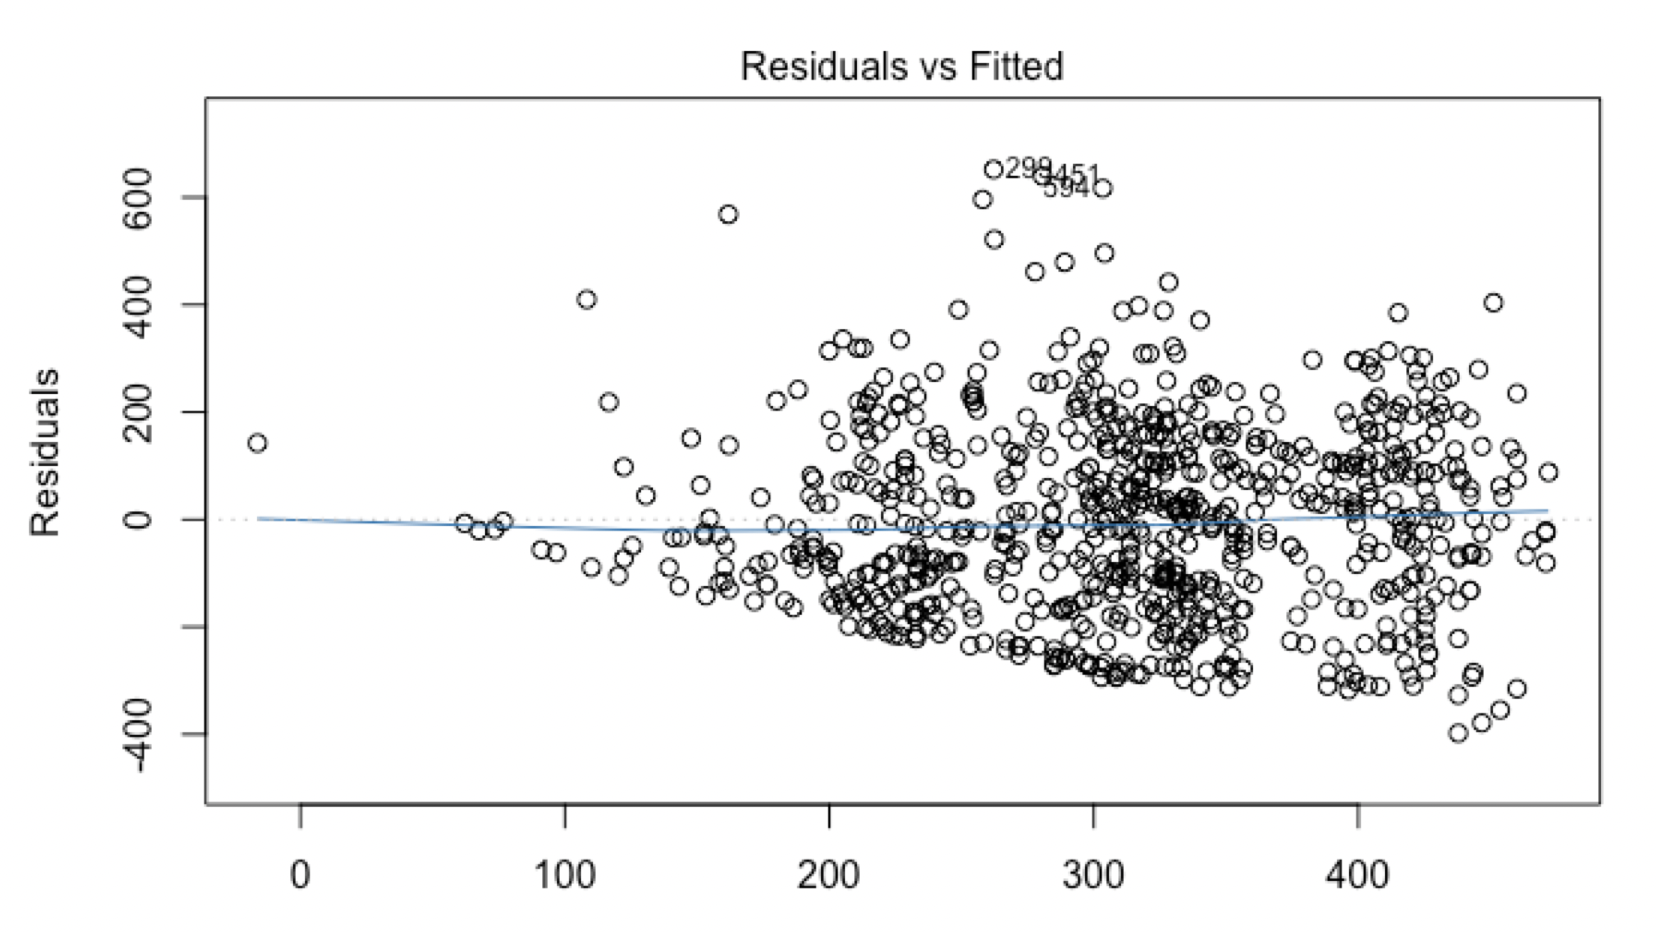
\includegraphics[width = 0.8\linewidth]{423Residual.png}
    \caption{Residual plot of the final model.}
    \label{residual}
\end{figure}

\begin{figure}[H]
    \centering
    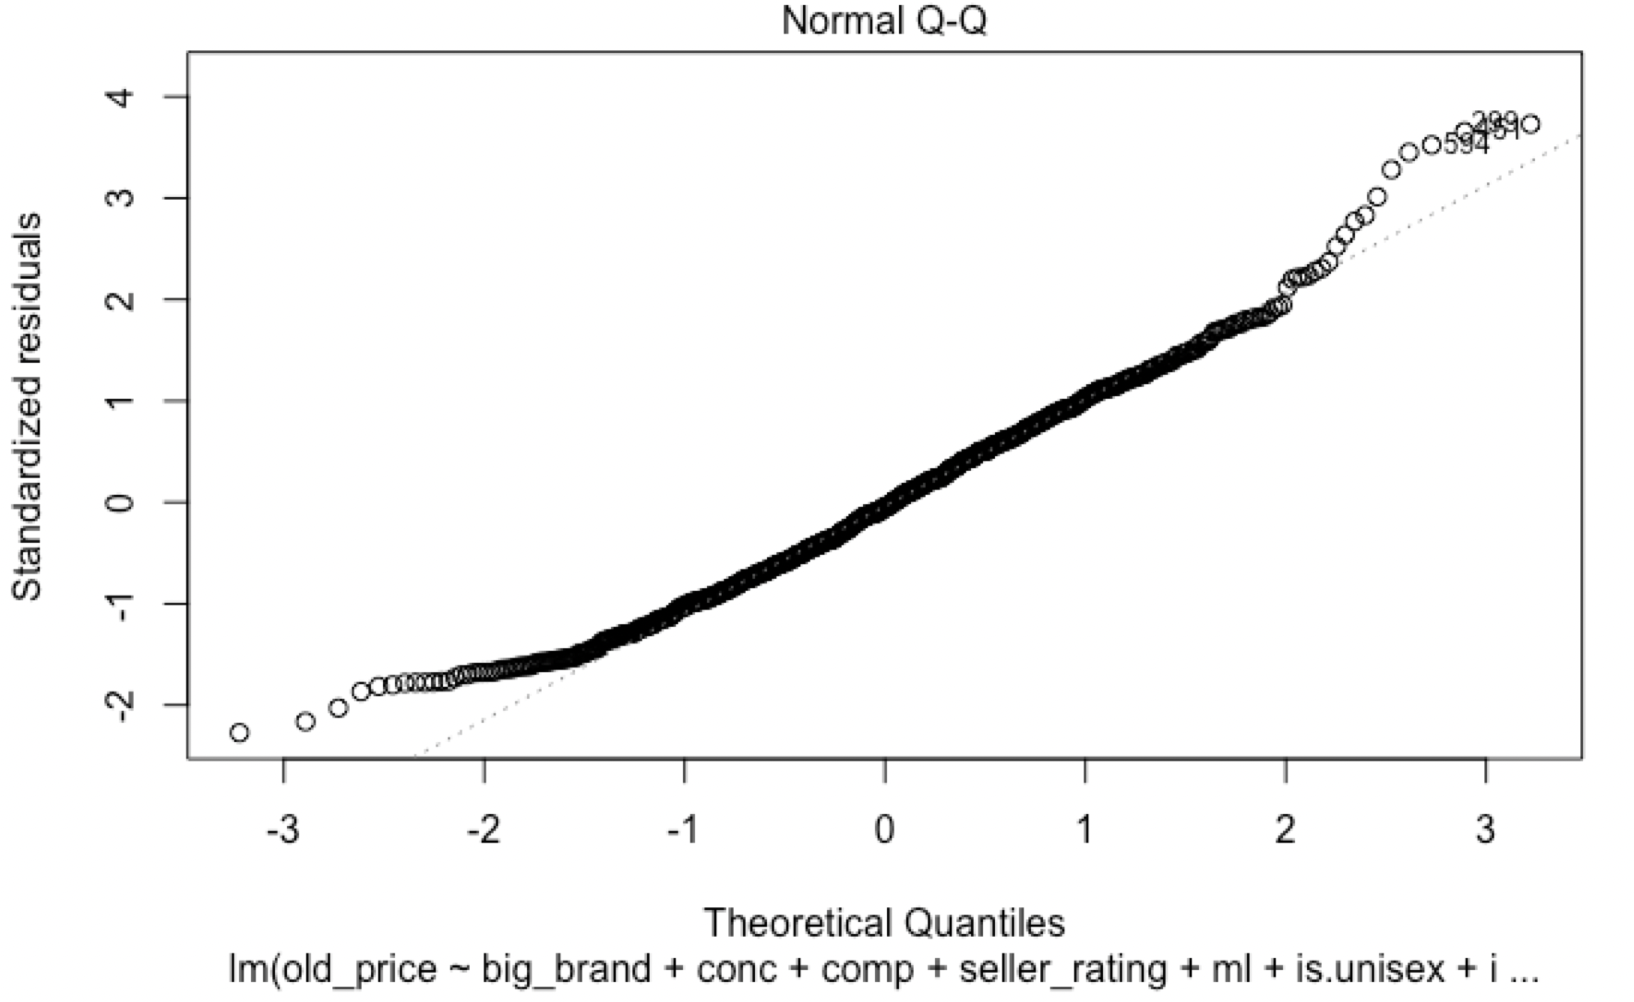
\includegraphics[width = 0.8\linewidth]{423QQPlot.png}
    \caption{Normal quantile-quantile plot of the final model.}
    \label{QQPlot}
\end{figure}

The residual standard error is 175.54, which means the model we proposed is a relatively 
good fit to the dataset. The adjusted R square is 0.17145, which means 17.145\% of the variation 
in the dataset can be explained by our model. Considering the overall simplicity of our model 
and the typically chaotic nature of perfume pricing, we would argue that the adjusted R square is 
already impressively high. The generalization error, Marllow’s Cp, AIC, and BIC of this model 
are all the lowest among all the models we have constructed while exploring; thus, this model 
has overall the best predictive power. Although typically AIC and BIC prefer different kinds of 
models due to the fact that these two criteria have different penalizing power on overfitting, our 
model achieved the lowest on both statistics. The 5-fold Cross Validation of this model gives a
mean squared prediction error of 31796, a relatively good improvement comparing to the mean 
squared prediction error of the 5-fold CV of the full model, which is 32891. In addition, all 7 
predictors included in our model are significant at a 5\% level, and these predictors’ coefficients 
largely reflect how market works in real life. Detailed explanation is provided in the Discussion Section.


A residual analysis is performed to test if the model assumptions are satisfied: we assumed the model to be 
$$\boldsymbol{y} = \boldsymbol{x\beta} + \boldsymbol{\epsilon},$$
where $\boldsymbol{\epsilon} \stackrel{iid}{\sim} \mathcal{N}(0, \sigma^2 \boldsymbol{I}_n)$. By checking the residual plot shown in Figure \ref{residual}, we would argue that the 0 mean assumption about errors is approximately satisfied. However, we suspect that the variance is not constant. Namely, the group of points with fitted value above 300 seems to share a constant variance, while the group of points with fitted value less than 300 seems to have a cone shape. Variance test established a p-value of 0.7152, which means there's no evidence supporting that there is a difference in variance across these two groups of points. Therefore, the constant variance assumption is also satisfied. The Durbin-Watson test gives a p-value of 0.0573, which means that there's no evidence supporting that the residuals are correlated. The independence assumption of errors is also satisfied. Lastly, by checking the normal QQ-plot shown in Figure \ref{QQPlot}, we argue that the normality assumption is also satisfied. 

\section{Discussion}

We shall interpret the coefficients from an economics perspective. Saudi Arabia has 
adopted a free market economic model. In such a model, the price of goods and services is only 
determined by demand and supply. Price increases as demand increases and decreases as supply 
increases, holding all other factors constant. In the following paragraphs, we will go over the 
coefficients of the seven predictors in our proposed model and discuss about how they make 
sense in a real-world context.

First is \texttt{big\_brand}, an indicator of whether the manufacturer of the perfume is a popular 
brand, with 1 means yes and 0 means no. In a free market, brand prestige is considered as a 
significant determinant of demand, namely higher brand prestige leads to higher demand. Since 
higher demand leads to higher price, holding other factors constant, the coefficient of \texttt{big\_brand}
should be a large positive number, which is 85.563, as expected. This means perfumes from popular 
brands are on average \$85.563 more expensive than perfumes from non-popular (niche) brands.

Second comes \texttt{is\_EDT}, which is short for concentration, a binary variable with 0 means 
EDP and 1 means EDT. EDT, short for Eau De Toilette, is more diluted than EDP, short for Eau 
De Parfum. Therefore, the cost of production of EDT perfumes are typically much lower than 
that of EDP perfumes. Cost of production is considered to be a significant determinant of supply; 
namely higher cost of production means lower supply. Since lower supply leads to higher price, 
holding other factors constant, we expect to see EDT perfumes have lower prices. That is exactly 
what observe—the coefficient of \texttt{is\_EDT} is -111.021, which means on average the price of 
EDT perfumes are \$111.021 cheaper than EDP perfumes.

For the same reason, the coefficient of \texttt{ml}, which is an indicator of the volume of the 
perfume, has a positive coefficient of 1.2119. This means on average, 1 ml increase in the 
volume of the perfume is associated with an \$1.2119 increase in the perfume’s retail price.

\texttt{seller\_rating} is related to loyalty, another determinant of demand. Better seller rating 
means the seller is more trustworthy and reliable, hence consumers will be more loyal to this 
seller. Therefore, higher seller rating is correlated with higher demand, and hence higher price, 
holding other factors constant. This explains the positive coefficient (56.859) of \texttt{seller\_rating}. 
Namely, for every 1 unit increase in seller rating, the price of the perfume is expected to increase 
by \$56.859 on average.

\texttt{is.unisex} is an indicator of whether the department of the perfume is unisex, with 1 
means yes and 0 means no. Saudi Arabia is not a LGBTQ friendly country; the laws there do not 
protect the rights of such groups and “non-binary gender” is not accepted by the law. Therefore, the number of potential buyers of unisex goods is little. Number of 
potential buyers is one of the determinants of demand, with larger number of potential buyers 
leads to higher demand and vice versa. Consequently, the coefficient of is.unisex is -146.30, 
meaning on average the price of unisex perfumes is \$146.30 cheaper than the price of non-unisex 
perfumes.

Perfume manufacturers typically want their products to have a feeling of structure and 
depth. This feeling can be created via either the easy way or the hard way. While the easy way 
involves using premium natural ingredients like Bulgarian rose essential oils, oud extracts, and 
ambergris, the hard way relies on the usage of “scent snapshots”—chemical synthetics like acid, 
calone, and aldehyde. Premium natural ingredients automatically create the feeling of structure 
and depth, while chemical synthetics are very simple and shallow. Therefore, it requires the 
stacking of multiple layers of “scent snapshots” to create the feeling of structure and depth, i.e., 
if we want the same level of feeling of structure and depth, “the hard way” will typically give 
more notes, and hence a higher \texttt{comp} score to the perfume comparing to “the easy way”. 
However, at the same time chemical synthetics, which have an average price of \$30-\$50 per 
ounce, are much cheaper than premium natural ingredients, as the price of those could go easily 
above \$1000 per ounce. Consequently, higher \texttt{comp} score is associated with lower cost of 
production; now, applying the logic mentioned previously, it means higher supply and hence 
lower price. Based on our model’s coefficient, for every 1 unit increase in comp, i.e., 1 more 
note contained in the perfume, the price of the perfume is expected to decrease by \$4.4408 on 
average.

Lastly, and the most interesting one is \texttt{is.fresh}, an indicator of whether a perfume is 
categorized to have a “fresh” scent, with 1 means yes and 0 means no. Fresh scent category is 
only created after the invention of calone, 30 years ago. So, fresh scent perfumes only have a 
history of around 30 years, while other scent perfumes like woody, floral, and oriental perfumes 
have over 1000 years of history. Therefore, the number of potential buyers of fresh scent 
perfumes is still small due to the fact that most people have not yet accepted “fresh” to be a 
perfume scent. Consequently, demand is lower and hence price is lower for fresh scent perfumes. 
Besides the “demand-side effect”, fresh scent perfumes are also related to a “supply-side effect”. 
Since the thing that brought fresh scent perfumes to life is a chemical synthetic—calone, and 
most fresh scent perfumes are created to capture the “aquatic smell”, fresh scent perfumes only 
use chemical synthetics as ingredients. Therefore, the cost of production is low and hence the 
supply is high; this means lower price when holding other factors constant. Combining both the
“demand-side effect” and the “supply-side effect”, fresh scent perfumes are automatically cheaper 
than the rest, namely by \$85.371 on average.

Another intrigue observation is that item rating has no correlation to price. This is 
understandable from a biopsychology perspective: when one smells a perfume, the olfactory 
bulbs and the end of the nostrils send feedback to the cortices of the brain; however, the signals 
do not only go to the cortices, but they also travel through hippocampus and hypothalamus, 
triggering memories and emotions that vary across individuals along the way. This means that 
“there are 1000 Acqua Di Gio’s in 1000 people’s noses”, yet there’s only one price. 
Consequently, item rating and price should be indeed uncorrelated.

In conclusion, based on our regression analysis, we find that the prestige of the brand contributes the most of the perfume's retail price, while the customer rating does not seem to be correlated with price. This potentially suggests that, one will always cost more in pursuit of the frontiers of the fashion trend, yet one might not need to spend much to own a perfume that one loves. Such a conclusion is only drawn from the Saudi Arabia perfume data set. In the future, we are interested in extending this work to data sets such as US Amazon/Sephora data for a more comprehensive and universal result.
\bibliographystyle{apalike} 
\bibliography{References.bib} 

\end{document}

\begin{comment}

\subsection{Data Cleaning}

In this section, we will elaborate the variables we considered in the model, how we clean the data, and how we transform the covariates for better analysis.

\subsubsection{Retail Price} \texttt{Price} is a quantitative variable. It is the outcome variable we would like to investigate.
\subsubsection{Base Notes \& Middle Notes} \texttt{Base note} and \texttt{Middle note} are two nominal categorical covariates. They suffer a similar problem as with \texttt{Scent}, thus our first step of data cleaning is to unify the covariate levels across data. Then, we noticed that there exists several hierarchical structures in the covariate levels, for instance,  \texttt{Bulgarian Rose} and \texttt{Rose}, \texttt{Africa Orange Flower} and \texttt{Orange Blossom}, etc. We then manually merged all lower branches of the same hierarchy to the highest one.
\subsubsection{Department} \texttt{Department} is a nominal categorical variable. This represents the designed gender of the perfumes. We merge category \texttt{Kid} with \texttt{Unisex} as they take up a smaller proportion of the perfumes and are non-distinguishable with gender. This results in the current three levels \texttt{Women}, \texttt{Men}, and \texttt{Unisex}.
\subsubsection{Perfume Brand} \texttt{Brand} is a nominal categorical covariate. Given the large amount of brands in the data set, we will categorize the perfume brand in the following manner. For a brand with more than 10 individual perfumes, we consider it as prevalent and consider it as a \texttt{Brand} level. For all the perfume brands with less than 10 individual perfumes, we will merge their perfumes under a \texttt{Brand} level named \texttt{Niche}, which represents for brands of niche perfume.
\subsubsection{Scents} \texttt{Scent} is a nominal categorical covariate. The original data seems to be directly crawled from the \textit{noon} web page, thus some of the same scents of perfume come in by different name and language (English, Arabian, Latin, etc.). We manually cleaned this category to make the covariate levels consist across our analysis. 
\subsubsection{Score} \texttt{Score} is a quantitative covariate. Such a variable is not contained in the original data set, and is developed and computed based on our personal consideration. We believe that the complexity of the perfumes (total number of raw ingredients contained in the perfume) as well as the value of raw ingredients contained in the perfume (luxurious ingredients such as Ambergris and Oud) will greatly impact the retail price of the perfume. Thus, we proposed the following score
\[\texttt{Score} = c \cdot \text{\# of ingredients} \cdot \text{weighted average of luxurious ingredients} \;.\]
We will elaborate the constant choice and criteria of luxury ingredient in the appendix.
\subsubsection{Seller} \texttt{Seller} is a nominal categorical covariate. We observed that over two thirds of \texttt{Seller} are directly affiliated with the \textit{noon} website (think it as \textit{Amazon's Choice}) and the rest come from a large variety of individual sellers. Thus, we will convert \texttt{Seller} into a binary covariate with two levels: \texttt{Noon} and \texttt{Non-Noon}.
\subsubsection{Volume} \texttt{Volume} is a nominal categorical covariate. Originally, it is a discrete quantitative covariate indicating the perfume's volume. We first removed the perfumes with volume $\leq 5ml$ to remove the perfume samples/testers. Then, we observed that the perfume volume concentrate on several values ($50ml, 150ml$, etc.) regardless of their brands. Thus, we think it is reasonable to convert \texttt{Volume} into a nominal categorical covariate, with each level corresponding to a specific volume value. 
\subsubsection{Concentration} \texttt{Concentration} is a nominal categorical covariate. The \texttt{Concentration} levels are eau de Cologne (\texttt{EDC}), eau de toilette (\texttt{EDT}), and eau de parfum (\texttt{EDP}), which are the concentration levels of perfumes ranked from low to high.
\subsubsection{Item Rating} \texttt{Item Rating} is a quantitative covariate indicating the customers' rating of the perfume, on a scale from $0$ to $5$.
\subsubsection{Seller Rating} \texttt{Seller Rating} is a quantitative covariate indicating the customers' rating of the Seller, on a scale from $0$ to $5$. 
\subsubsection{Total Sellers} \texttt{Total Sellers} is a discrete quantitative covariate indicating the number of customers' rating on the seller.
\end{comment}

